\documentclass{winnower}
\usepackage{indentfirst}
\usepackage{graphicx}
\usepackage{caption}
\usepackage{subfigure}
\usepackage{xcolor}
\usepackage{float}
\usepackage[section]{placeins}
\usepackage{multirow}
\usepackage{booktabs}
\setlength{\belowcaptionskip}{-0.5cm}

\begin{document}

\title{Homework6 report}

\author{Haoyu Guan}

\affil[1]{Questrom School of Business, Boston University}







\date{2020.02.11}

\maketitle




%-------------------------------------------------%
\section{Simulation in the Heston Model:}
%-------------------------------------------------%


\indent Suppose that the underlying security SPY
evolves according to the Heston model. That is, we know its dynamics are defined by the
following system of SDEs:

%\vspace{12 pt}
$$\begin{aligned}
d S_{t} &=(r-q) S_{t} d t+\sqrt{\nu_{t}} S_{t} d W_{t}^{1} \\
d \nu_{t} &=\kappa\left(\theta-\nu_{t}\right) d t+\sigma \sqrt{\nu_{t}} d W_{t}^{2} \\
\operatorname{Cov}\left(d W_{t}^{1}, d W_{t}^{2}\right) &=\rho d t
\end{aligned}$$


You know that the last closing price for SPY was $282 .$ You also know that the dividend yield for SPY is $1.77 \%$ and the corresponding risk-free rate is $1.5 \%$

Using this information, you want to build a simulation algorithm to price a knock-out option on SPY, where the payoff is a European call option contingent on the option not being knocked out, and the knock-out is an upside barrier that is continuously monitored. We will refer to this as an up-and-out call.
\\

This payoff can be written as:
$$
c_{0}=\mathbb{E}\left[\left(S_{T}-K_{1}\right)^{+} 1_{\left\{M_{T}<K_{2}\right\}}\right]
$$
where $M_{T}$ is the maximum value of $S$ over the observation period, and $K_{1}<K_{2}$ are the strikes of the European call and the knock-out trigger respectively.
\\


\textbf{1. Find a set of Heston parameters that you believe govern the dynamics of SPY. You
may use results from a previous Homework, do this via a new calibration, or some other
empirical process. Explain how you got these and why you think they are reasonable.}
\\
I would set the Heston model parameters like this below:
$$\sigma=1.9$$
$$\nu_0=0.05$$
$$\kappa=3.65$$
$$\rho=-0.8$$
$$\theta=0.07$$

Those parameters' value are from the previous homework.

\newpage
\textbf{2.Choose a discretization for the Heston SDE. In particular, choose the time spacing,
$\Delta T$ as well as the number of simulated paths, $N .$ Explain why you think these choices will lead to an accurate result.}
\\

I set N=100000 paths and M=1000 timeparts.

\begin{figure*}[!h]
\begin{center}
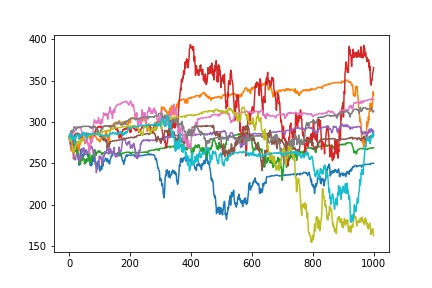
\includegraphics[scale=0.7]{1_1.jpg}
\caption
{path generation}
\label{fig:f1}
\end{center}
\end{figure*}

I think this is good enough because the N and M are big enough to make the mesh finer.
$$c_0=22.443401619891834$$


\textbf{3.Write a simulation algorithm to price a European call with strike $K=285$ and time to expiry $T=1 .$ Calculate the price of this European call using FFT and comment on the difference in price.}
\\
$$c_0=18.523241425992897$$

I think it is right for a lower price.Because the simulation methods avoid those situation that volatility is negative.
\\


\newpage
\textbf{4. Update your simulation algorithm to price an up-and-out call with $T=1, K_{1}=285$ and $K_{2}=315 .$ Try this for several values of $N .$ How many do you need to get an accurate price?}
\\

when N=100000
$$c_0=1.6594169853560121$$

\begin{figure*}[!h]
\begin{center}
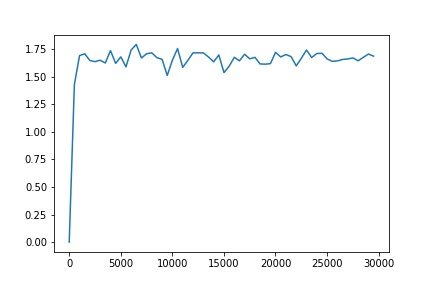
\includegraphics[scale=0.7]{1_2.jpg}
\caption
{converge 1}
\label{fig:f1}
\end{center}
\end{figure*}





\textbf{5. Re-price the up-and-out call using the European call as a control variate. Try this for several values of $N .$ Does this converge faster than before?}
\\
$$c_0=1.6871799736634712$$


\begin{figure*}[!h]
\begin{center}
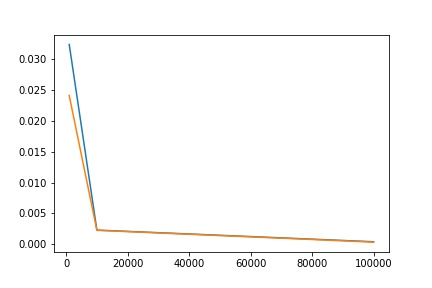
\includegraphics[scale=0.7]{1_3.jpg}
\caption
{converge 2}
\label{fig:f1}
\end{center}
\end{figure*}






\end{document}
